\documentclass[twoside]{article}


\usepackage{amssymb}
\usepackage[table,xcdraw]{xcolor}
\usepackage{amsmath}
\usepackage[brazilian]{babel}
\usepackage[utf8x]{inputenc}
\usepackage[sc]{mathpazo}
\linespread{1.05}
\usepackage{microtype}
\usepackage[hang, small,labelfont=bf,up,textfont=it,up]{caption}
\usepackage{lettrine}
\usepackage{graphicx}

\usepackage[hmarginratio=1:1,top=20mm,bottom=35mm,right=15mm,left=15mm,columnsep=20pt]{geometry}
\usepackage{multicol}
\usepackage{booktabs}
\usepackage{float}
\usepackage{subfigure}
\usepackage{paralist}
\usepackage{hyperref}
\usepackage{abstract}
\renewcommand{\abstractnamefont}{\normalfont\bfseries}
\renewcommand{\abstracttextfont}{\normalfont\small\itshape}
\usepackage{titlesec}
\renewcommand\thesection{\Roman{section}}
\renewcommand\thesubsection{\Roman{subsection}}
\titleformat{\section}[block]{\large\scshape\centering}{\thesection.}{1em}{}
\titleformat{\subsection}[block]{\large}{\thesubsection.}{1em}{}

\usepackage{fancyhdr}
\pagestyle{fancy}
\fancyhead{}
\fancyfoot{}
%AQUI VOCE COLOCA A SIGL do grupo
\fancyhead[C]{Teoria Geral da Administração $\bullet$ Projeto de Pesquisa $\bullet$ \date{\today} }
\fancyfoot[RO,LE]{\thepage} \newenvironment{Figure}
  {\par\medskip\noindent\minipage{\linewidth}}
  {\endminipage\par\medskip}

% AQUI VOCÊ COLOCA O TÍTULO DO SEU EXPERIMENTO.

\title{\vspace{-10mm}\fontsize{18pt}{20pt}\selectfont\textbf{Sistemas Tecnológicos na Gestão do Sistema Único de Saúde (SUS)}}

% AQUI VOCE COLOCA O NOME DOS AUTORES DO TRABALHO

\author{
\large
\textsc{Daniel Terra Gomes,} \textsc{Estefânio Silva Ribeiro}\\[2mm]
%\textsc{Estefânio Silva Ribeiro}\\[2mm]
\large Universidade Estadual do Norte Fluminense Darcy Ribeiro – UENF\\[2mm]
\smallsize \href{mailto:danielterra@pq.uenf.br}{danielterra@pq.uenf.br}\\[2mm]
\smallsize \href{mailto:20201100011@pq.uenf.br}{20201100011@pq.uenf.br}\\[2mm]
%\smallsize\date{\today}
%\vspace{2mm}
}
\date{}

\begin{document}
\maketitle

\thispagestyle{fancy}

%___________________________________
%\raggedleft\date{\today} % Leave empty to omit a date

\begin{abstract}
  \textbf{Este artigo tem como objetivo compreender os desafios enfrentados pelos formuladores de políticas e gestores do Sistema Único de Saúde (SUS) para garantir a disponibilidade geográfica e acessibilidade dos serviços médicos. A análise foi norteada por um modelo explicativo do trabalho em saúde. Dos problemas principais foram identificados: (i) falta de médicos, (ii) distribuição insuficiente desses profissionais, (iii) distribuição insuficiente de medicamentos entre níveis de atenção à saúde e entre zonas geográficas. 
Visto que, o sistema de saúde brasileiro passou por mudanças significativas nos últimos 30 anos. Este artigo, também descreveu as tendências em atendimento ambulatorial e hospitalar, níveis de pessoal e uso de serviços de saúde durante este período. Ademais, houve uma análise das barreiras de acesso ao tratamento de doenças com base nos processos administrativos de medicamentos.
  Conclui-se que, para muitas regiões geográficas a abordagem de atendimento virtual para consultas com o médicos, não só para a apresentação de resultados médicos, como também prescrição de medicamentos, possibilitará a população brasileira a ter maior aproveitamento do SUS.}
\end{abstract}

\vspace{2mm}

\textbf{Palavras-chaves}: SUS, TI, Sistema Único de Saúde, Tecnologia, Dados, Sistemas.
%
\vspace{0.5cm}
\begin{multicols}{2}

  \section{Introdução}

O Sistema Único de Saúde (SUS) inclui um sistema complexo de conexões de serviços públicos e privados. Foi idealizado em 1988 a partir do Movimento Sanitário Brasileiro, garantindo a saúde como direito do cidadão e dever do Estado, com a saúde pautada nos princípios da universalidade, equidade e integralidade \cite{Miranda_2017}.
Essa idealização se torna ainda mais difícil. Sabendo que, o Brasil é um país extenso territorialmente e desigual economicamente.

Dessa forma, o emprego de sistemas tecnológicos no setor de saúde têm permitido, no Brasil, agilizar e proporcionar mais inteligência nos atendimentos pelo SUS, visto que, pela alta demanda de atendimentos, uma forma de agilizar o processo faz-se mister, pois, dados mais atualizados mostram que em 2015 havia 1,95 médicos a cada mil habitantes. Porém, sabe-se que existem diversos problemas na aplicação real desta tecnologia da informação, desde falta de preparação dos funcionários à precariedade tecnológica dos pacientes, somados a uma má gestão que não só afeta o financeiro como também, diretamente, a saúde da população.

Em 1990 tinha 1,12 médicos a cada mil habitantes, e em 2010 esse número foi para 1,86. O número ideal de médicos para uma população é uma contagem complexa. Tendo que ser levado em conta características como (demografia social, idade, gênero sexual); processos de trabalho (produtividade, carga de trabalho, serviço não clínico e variações no nível de atividade), características do sistema de saúde em vigor no país (por exemplo, cobertura e tipo
dos serviços oferecidos), e as condições da população (socioeconômicas e epidemiológicas) \cite{Oliveira_2017}.

Mormente, é fulcral ressaltar a importância da saúde para o ser vivo, e quando o assunto remete ao sistema de saúde, a prioridade consiste na qualidade, quantidade e eficácia dos atendimentos. De acordo com os dados do Mapa Assistencial, publicado pela Agência Nacional de Saúde Suplementar (ANS), foram realizados pelos SUS 1,57 bilhão de procedimentos como consultas, exames e internações somente no ano de 2018. Todavia, muitos desses atendimentos poderiam ser executados com maior eficiência através do uso de sistemas tecnológicos, visto que o uso dos mesmo facilitam o acesso às informações do paciente através de um banco de dados com todos os atendimentos que o cidadão recebeu em qualquer rede pública de saúde do Brasil. Esses dados proporcionam maior agilidade, onde por intermédio do mesmo, sabe-se se o paciente em questão tem algum tipo de alergia a medicamentos, histórico de atendimentos e etc.

No entanto, como mencionado anteriormente, a execução dessa tecnologia está longe de ser perfeita. Os hospitais que têm acesso a essa tecnologia da informação não fazem o completo uso da mesma, onde atualmente utilizam-se apenas para registrar o atendimento dos pacientes. Apesar desta ser sua função primária, a gama de possibilidades que esse sistema fornece está além de apenas agilizar o atendimento e portabilizar os dados através da rede, possibilidades essas que afetam diretamente o lado financeiro, ambiental e da saúde \cite{Oliveira_2017}, \cite{Pinheiro_Filho_2012}.

    Algumas das possibilidades para aplicação do sistema de tecnologia, seriam:
    \begin{itemize}
    \item Solicitação de leitos: O hospital verifica no sistema se existem outros leitos nas proximidades, ou onde teria um mais próximo.
    \item Reabastecer estoque: Saber através de oferta e demanda, a quantidade que cada posto de saúde necessita. Visto que alguns hospitais têm demanda variada de remédios.
    \item Utilizar a demanda de remédios como medida para compra: Por meio da oferta e demanda dos remédios, o governo poderia saber quais remédios estão sendo mais solicitados que outros, e dar prioridade a esses, e diminuir a compra dos que têm pouca saída. Através desse método, os estoques terão os remédios sem falta e o dinheiro não será “desperdiçado” com remédios com baixa solicitação.
    \item Redução de lixo hospitalar: como citado, existem remédios com alta compra com baixa demanda, e quando eles não tem mais serventia por conta da validade ter vencido, esses remédios se tornam lixo hospitalar. Esse lixo hospitalar, que muita das vezes é mal conduzido, gera danos ambientais, que mais uma vez pesam no financeiro.
    \end{itemize}
\begin{footnotesize}
*Este estudo se propõe a analisar a organização do Sistema Único de Saúde no pacto federativo brasileiro, apontando para
formas possíveis de garantir os princípios e diretrizes que a norteiam. Ademais, focando nos processos de gestão tendo o uso da tecnologia como principal ferramenta que busca uma igualdade ao acesso à rede de saúde.
\end{footnotesize}
  
\iffalse
  \section{Hipótese}



  %Exemplo Tabela 1

  \begin{table*}
    \centering
    \caption{Título da tabela}
    \begin{tabular}{cc c c c c}
      \hline
      Variável            & $g_i^1$ & $g_i^2$ & $g_i^3$ & $g_i^4$ & $g_i^5$ \\
      \hline
      $Re(\lambda)_{max}$ & -0.01   & -0.005  & -0.001  & -0.0005 & -0.0001 \\
      $u_{max}$           & 0.85    & 0.90    & 1       & 1.5     & 2       \\
      $t_{est}^{max}$     & 14      & 16      & 18      & 21      & 25      \\
      $noise_{max}$       & 0.5     & 0.9     & 1.2     & 1.4     & 1.5     \\
      $u_{nom}$           & 0.5     & 0.7     & 1       & 1.5     & 2       \\
      $t_{est}^{nom}$     & 10      & 11      & 12      & 14      & 15      \\
      \hline
    \end{tabular}
  \end{table*}

  Curabitur sed ante egestas, vehicula tortor quis, faucibus lorem. Nulla vel sollicitudin quam. Pellentesque non nunc at magna malesuada ullamcorper quis ut nunc. Suspendisse ac molestie turpis. Aliquam ac convallis augue. Praesent commodo, dolor at aliquam vehicula, augue nulla facilisis massa, sed pharetra urna nunc sit amet metus. Vestibulum sit amet molestie nibh, in congue urna. Curabitur condimentum sagittis consequat. Aliquam mollis eros nisl, in ultricies ante lacinia at. Orci varius 

%  \begin{figure}[H]
%    \centering
%    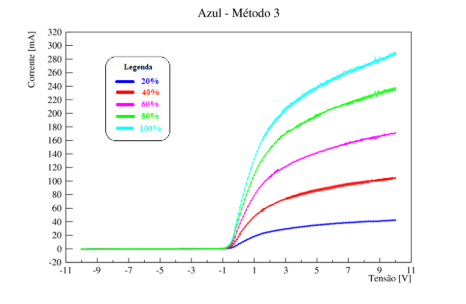
\includegraphics[scale=0.75]{figurateste.png}
%    \caption{Legenda da figura.}
%    \label{fig}
%  \end{figure}


  \section{Justificativa}
  
    Phasellus ac iaculis neque. Cras ante magna, cursus eget consectetur id, rutrum sed libero. Fusce at nulla ut risus iaculis hendrerit at eu ex. Praesent pulvinar sem sed ligula gravida, a maximus leo sagittis. Integer efficitur eros eget tempus porttitor. Sed justo dolor,
      Proin et sem vitae ante porttitor viverra id et turpis. Aenean mollis eros vel ante tempor, ut elementum enim aliquam. Nam ut ante tempor, dapibus sem sit amet, dictum ipsum. Phasellus libero libero, vulputate nec iaculis quis, sagittis molestie magna. Morbi risus justo, ornare quis orci in, scelerisque convallis lacus. In congue pulvinar tincidunt. Aenean auctor lacus eu posuere sollicitudin. Maecenas a pulvinar ex, id aliquam tellus. Fusce scelerisque massa ex. Pellentesque placerat ac purus non ultricies. Maecenas sed feugiat nulla, vel pellentesque ipsum. Ut id imperdiet libero
      
    \section{----}
      
\fi      


  
  \section{Resultados e Discussão}
  
O desenvolvimento do SUS nos últimos 30 anos também está relacionado a mudanças nos recursos 
humanos. A disponibilidade de trabalhadores qualificados da
Saúde em geral e mais especificamente
nas unidades de Atenção Básica (AB), onde é possível avaliar o aumento da oferta desses recursos e os efeitos da
diretrizes específicas, como a Política Nacional de
Atenção Básica e Programa Mais Médicos.
As figuras 1, 2 e 3 fornecem informações sobre o número total de médicos e a proporção de médicos por 1.000
residentes ao longo do tempo, a participação de médicos, enfermeiras e dentistas que compõe a equipe.
O SUS e a atuação desses profissionais na AB.



\iffalse


  \begin{table*}[ht]
    \centering
    \caption{Legenda da tabela }
    \label{tabladeseables}
    \begin{tabular}{lcccccc}   \hline
      Controlador       & $Re(\lambda)_{max}$ & $u_{max}$   & $t_{est}^{max}$ & $noise_{max}$ & $u_{nom}$   & $t_{est}^{nom}$ \\ \hline
      B23               & INA                 & INA         & INA             & INA           & AD          & AIND            \\
      M23               & AD                  & AD          & AD              & T             & AD          & AIND            \\
      PPGA23            & \textbf{AD}         & \textbf{AD} & \textbf{AD}     & \textbf{AD}   & \textbf{AD} & \textbf{AD}     \\
      \hline
      W34               & AD                  & AD          & D               & T             & AD          & IND             \\
      M34               & AD                  & AD          & D               & AD            & AD          & AD              \\
      \textbf{PPGA23}*  & \textbf{AD}         & \textbf{AD} & \textbf{AD}     & \textbf{AD}   & \textbf{AD} & \textbf{AD}     \\
      \textbf{PPGA34}   & \textbf{AD}         & \textbf{AD} & \textbf{AD}     & \textbf{AD}   & \textbf{AD} & \textbf{AD}     \\
      \hline
      J45               & AD                  & IND         & AD              & IND           & AD          & AD              \\
      M45               & AD                  & AD          & IND             & T             & AD          & IND             \\
      \textbf{PPGA23}** & \textbf{D}          & \textbf{AD} & \textbf{D}      & \textbf{T}    & \textbf{AD} & \textbf{D}      \\
      \textbf{PPGA34}** & \textbf{AD}         & \textbf{AD} & \textbf{D}      & \textbf{D}    & \textbf{AD} & \textbf{D}      \\
      \textbf{PPGA45}   & \textbf{AD}         & \textbf{AD} & \textbf{AD}     & \textbf{AD}   & \textbf{AD} & \textbf{D}      \\
      \hline
    \end{tabular}
  \end{table*}


\fi
  \begin{figure}[H]
    \centering
    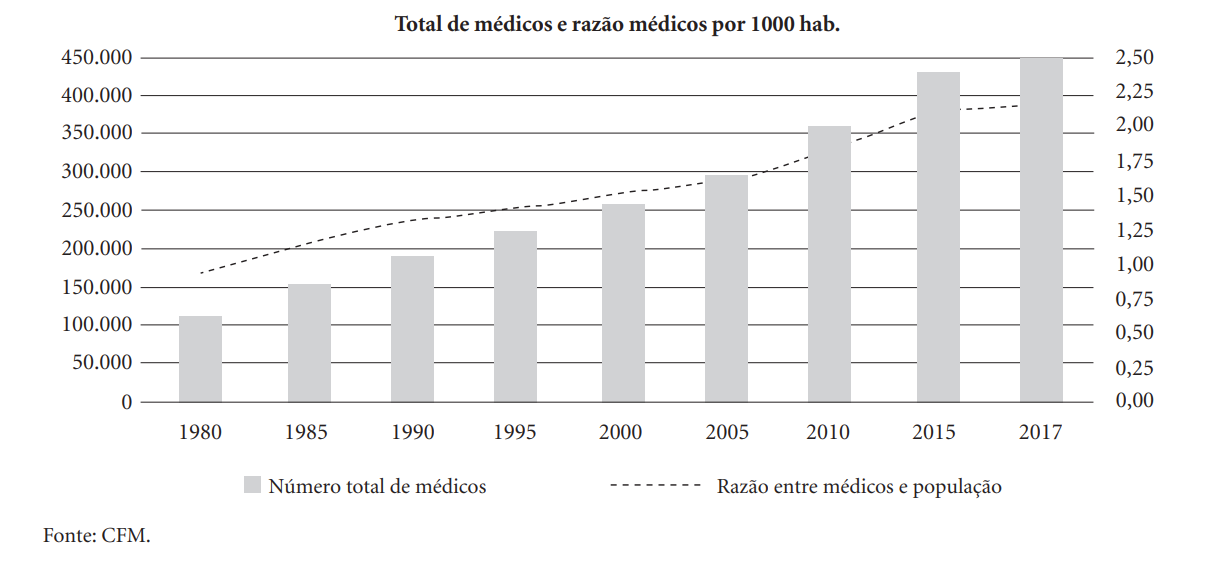
\includegraphics[scale=0.35]{mil medicos a cade .png}
    \caption{Evolução dos Recursos Humanos.}
    \label{fig2}
  \end{figure}
  
    \begin{figure}[H]
    \centering
    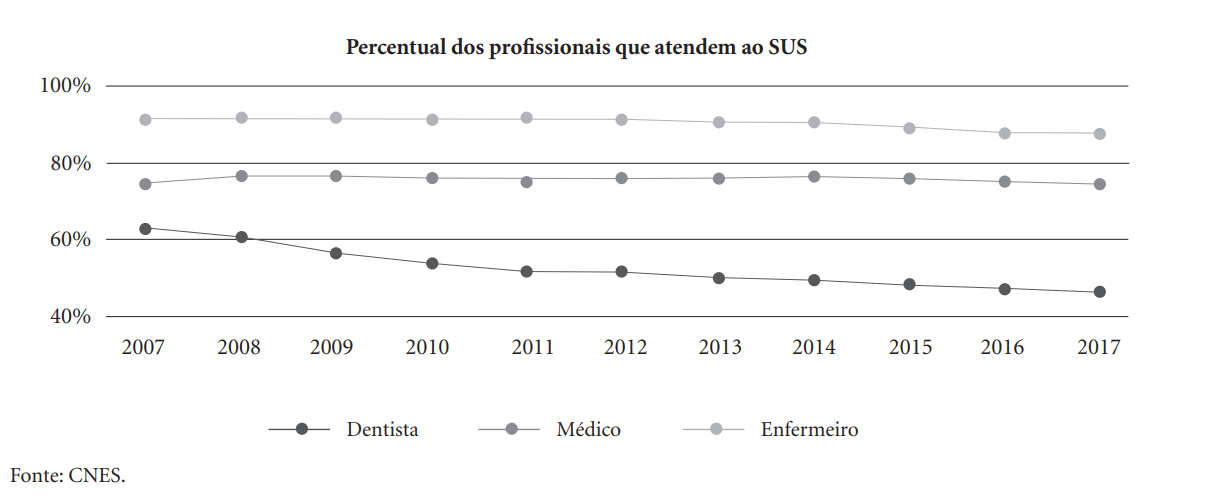
\includegraphics[scale=0.35]{medicos no sus.png}
    \caption{Evolução dos Recursos Humanos.}
    \label{fig2}
  \end{figure}
  
    \begin{figure}[H]
    \centering
    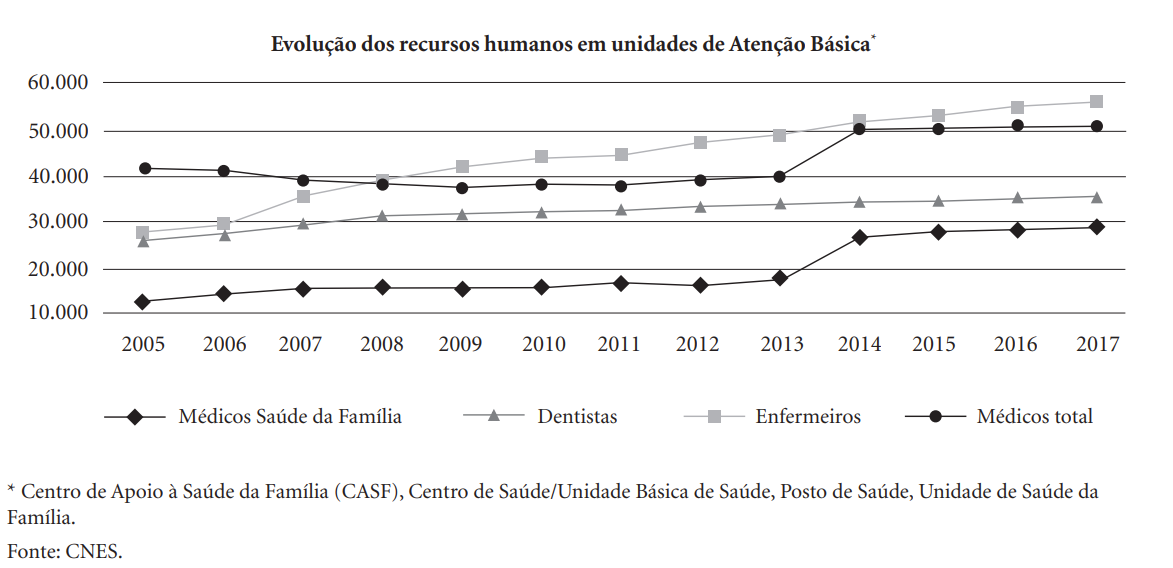
\includegraphics[scale=0.35]{atencao basica.png}
    \caption{Evolução dos Recursos Humanos.}
    \label{fig2}
   \end{figure}
 \begin{footnotesize}  
    *Dados: \cite{Viacava_2018}.
\end{footnotesize}  
 
O número de médicos é de aproximadamente
111.000 em 1980 para 447.000 em 2017. O CNES
registros mostram que o número de enfermeiras aumentou de cerca de 90.000 em 2007 para 230.000 em 2017, enquanto o número de dentistas foi de 78.000 em 2007
para 127.000 em 10 anos.
A proporção de médicos por mil habitantes também aumentou significativamente, pois o número de especialistas cresce mais rápido do que o da população. No
Em 1980 a taxa era inferior a 1 médico por mil habitantes (0,94) e chegava a 2,15 médicos em 2017
por mil habitantes. O maior crescimento ocorreu
entre 2005 e 2015, com um aumento de 1,6 para
2,15, ligeiramente superior à variação na 25ª
nos últimos anos.

Entretanto, um dos desafios desse cenário é a multiplicidade de modalidades de contratação, algumas delas precárias, pois não houve padronização da política de pessoal
Dificuldades de contratação e retenção de trabalhadores qualificados em muitos locais. Portanto, é importante destacar as acentuadas desigualdades regionais em termos de disponibilidade de trabalhadores qualificados que fazem parte da ampla gama de persistentes desigualdades sociais, econômicas e espaciais. \cite{Viacava_2018}


  \section{Discussões Finais}
A  difusão do SUS nos últimos 30 anos foi moldado por importantes
mudanças na atenção à saúde da população. A
ampliação do leque de serviços e especialistas
vinculado ao SUS e as opções de acessos,
mudanças no comportamento de uso estão entre os elementos de mudança mais importantes. Por outro lado, é importante destacar os desafios históricos
isso inclui relações público-privadas
na prestação de serviços de saúde, os mais destacados
desigualdades regionais e subfinanciamento.

Além disso, é de fundamental importância a superação do caráter formal das normas e diretrizes instituídas desde a implantação do SUS, promover a articulação das três esferas de governo para atuar como coletivo capaz de consolidar as redes de saúde e reduzir as desigualdades que caracterizam a sociedade brasileira.
Diante do desafio de subfinanciar o sistema de saúde em um cenário de crise política e financeira, é preciso resgatar os ideais que legitimaram o movimento sanitário brasileiro. O momento clama por uma ação de resistência em defesa do SUS para garantir a universalidade, inegavelmente a maior conquista social do povo brasileiro.

Ademais, o acesso a medicamentos para o tratamento de doenças do SUS requer procedimentos administrativos complexos e onerosos. Para as barreiras de acesso nele identificadas é destado o atraso e a burocracia do
procedimentos administrativos, a dificuldade de prescrição do comprimidos, e a prevalência de processos não concluídos que dificulta o acesso aos tratamentos, um enorme fardo sobre o financiamento da saúde pública e as despesas salariais dos pacientes e seus familiares. Porque o principal motivo da não concessão foi o não acesso dos pacientes a esses profissionais de saúde, por outro lado também há o desconhecimento do o Protocolo Clínico e Diretrizes Terapêuticas  por parte dos médicos destacando a necessidade de promover o treinamento dos prescritores para melhorar o acesso ao uso de certos medicamentos necessários em fase inicial de doenças.



\bibliographystyle{plain} % We choose the &quot;plain&quot; reference style
\bibliography{refs} % Entries are in the &quot;refs.bib&quot; file</code></pre> Entries are in the &quot;refs.bib&quot; file</code></pre>


\end{multicols}
\end{document}
